\section{The Space of Pentatonic Scales}
Our usual tonal system consists of 12 halftone steps C-C$\sharp$-D-E$\flat$... Each tone occurs exactly once in every octave. A nice way of visualizing this collection of tones is to arrange them in a circle and neglect the octave information. The image on the left shows the twelve notes with the usual distribution of black and white keys of a piano. The white circles form the material of the well-known C-major scale. But just playing the black notes also sounds interesting. They form a so called pentatonic scale: a collection of five notes within an octave. Forming melodies with them sounds a bit like modal music from the Far East. Rotating the pattern cyclically creates 12 similar sounding pentatonic scales.

\begin{figure}[h]
\centering
\begin{subfigure}{0.45\textwidth}
\centering
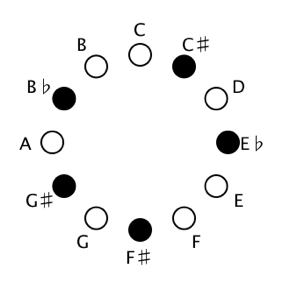
\includegraphics[width=0.9\textwidth]{PentatonicScales_1}
\end{subfigure}
\begin{subfigure}{0.45\textwidth}
\centering
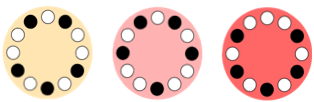
\includegraphics[width=\textwidth]{PentatonicScales_2}
\end{subfigure}
\end{figure}

There are plenty of other ways to select exactly 5 notes out of the 12 notes in our tonal system. However, if we want to restrict ourselves to more or less equally distributed selections we can in addition require that no two ``neighboring'' notes are selected. Under these conditions there are, depending on rotation, exactly two more such arrangements of five tones. Each of them can occur in 12 different rotations (see picture).

\paragraph{The Music:} The pentatonic scales above have a kind of free floating sound that has no specific appeal of major or minor. Some of them sound very peaceful (the yellow one), some of them are full of tension. These scales were extensively used by the composers of the impressionistic epoch such as Debussy. They are used to create very colorful sounds invoking vivid pictures of other cultures. Debussy, for example became interested in pentatonic scales after hearing Gamelan Music from Java and Bali.

\paragraph{The Math:} The picture shows the space of all the above-mentioned halftone free pentatonic scales. Each of the three types occurs in 12 rotational positions. In the picture the scales are arranged in such a way that two of them are connected by an arc if they differ exactly by one halftone step. You see the ``space of pentatonic scales''.

\paragraph{The Exhibit:} In the Exhibit, a piece by a classical composer (Mozart, Bach, Debussy, Liszt, and others) can be chosen for playing. But the piece is not played according to notation. You choose a pentatonic scale and each note of the piece is replaced by the nearest tone on the scale. By tapping the rosettes, you can walk around and move from one pentatonic scale to another. Through this, you can create your own pieces of impressionistic music.

\begin{figure}
\centering
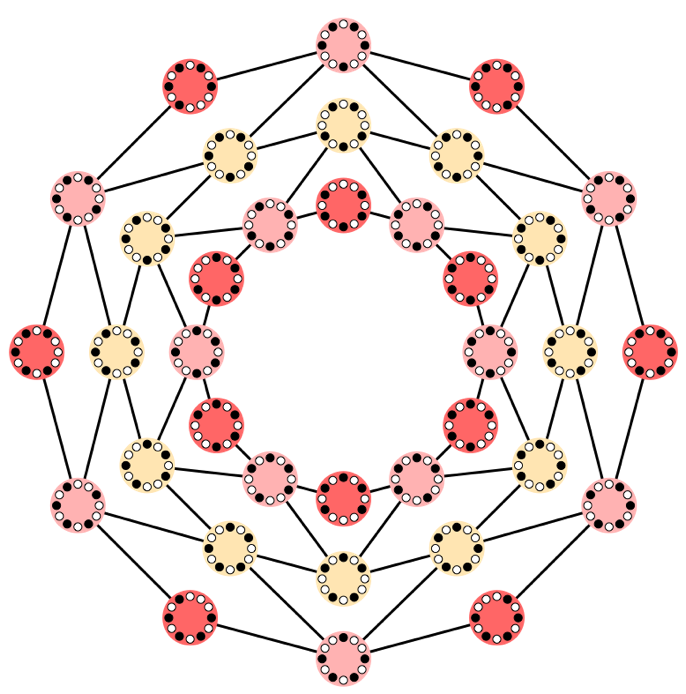
\includegraphics[width=0.6\textwidth]{PentatonicScales_3}
\end{figure}

\begin{sectcredits}
\item[Author of this exhibit:] Jürgen Richter-Gebert (Technical University of Munich)
\item[Acknowledgements:] Patrick Wilson and Aaron Montag (Sound Engine). Based on CindyJS.org
\item[Text:] Jürgen Richter-Gebert (TU Munich)
\item[Music:] Bach. Prelude and Fugue in C major BWV 846 / Mozart, Sonata No. 16 C major (Sonata facile), KV 545 / Liszt, Hungarian Rhapsody No 9 / Chopin, Prelude No 4  in e minor. Recorded by Bernd Krueger, Germany.
Gershwin. Rhapsody in Blue / Debussy, Arabesque 1 / Debussy, Images -- Reflets dans l'eau. Performed by Katsuhiro Oguri, Japan.
\end{sectcredits}
